% 封面。main.tex 用 \input 把它放在第一页；根目录的 cover.tex 也用它单独生成 cover.pdf。
% 版式仿照《Computer Architecture: A Quantitative Approach》第 6 版：
%   上半部白底，作者名一行，下面是大号细衬线的英文书名和中文书名，都靠右对齐；
%   中间一条深红色的横带写副标题，压在照片的上沿；
%   下半部是一张黑白照片（figures/cover_gray.png，由 tools/png_gray.py 生成），一直铺到页面底边；
%   中文书名左边的空白处贴着一张小小的彩色猫狗大战（figures/catdog.png）；
%   右上角竖着一个红色的小标签，左下角是“出版社”的标志。

% 书名、作者都在这里改
\providecommand{\CoverEnTitle}{C LANGUAGE}
\providecommand{\CoverEnSubtitle}{A Lazy Approach}
\providecommand{\CoverZhTitle}{教猫狗学编程}
\providecommand{\CoverAuthor}{whensungoesdown}
\providecommand{\CoverEdition}{First Edition}

\definecolor{coverred}{RGB}{190,30,45}
\definecolor{covergray}{RGB}{90,90,90}
\newfontfamily\coverfont{texgyrepagella}[
  Extension=.otf, UprightFont=*-regular, BoldFont=*-bold,
  ItalicFont=*-italic, BoldItalicFont=*-bolditalic]
\setCJKfamilyfont{coverkai}{FandolKai-Regular}[Extension=.otf]

\begin{tikzpicture}[remember picture, overlay, every node/.style={inner sep=0pt}]
  \coordinate (TR) at (current page.north east);

  % ---- 下半部：黑白照片，从横带的上沿一直铺到页面底边 ----
  \begin{scope}
    \clip ($(current page.north west) + (0,-164mm)$) rectangle (current page.south east);
    \node[anchor=south] at (current page.south)
      {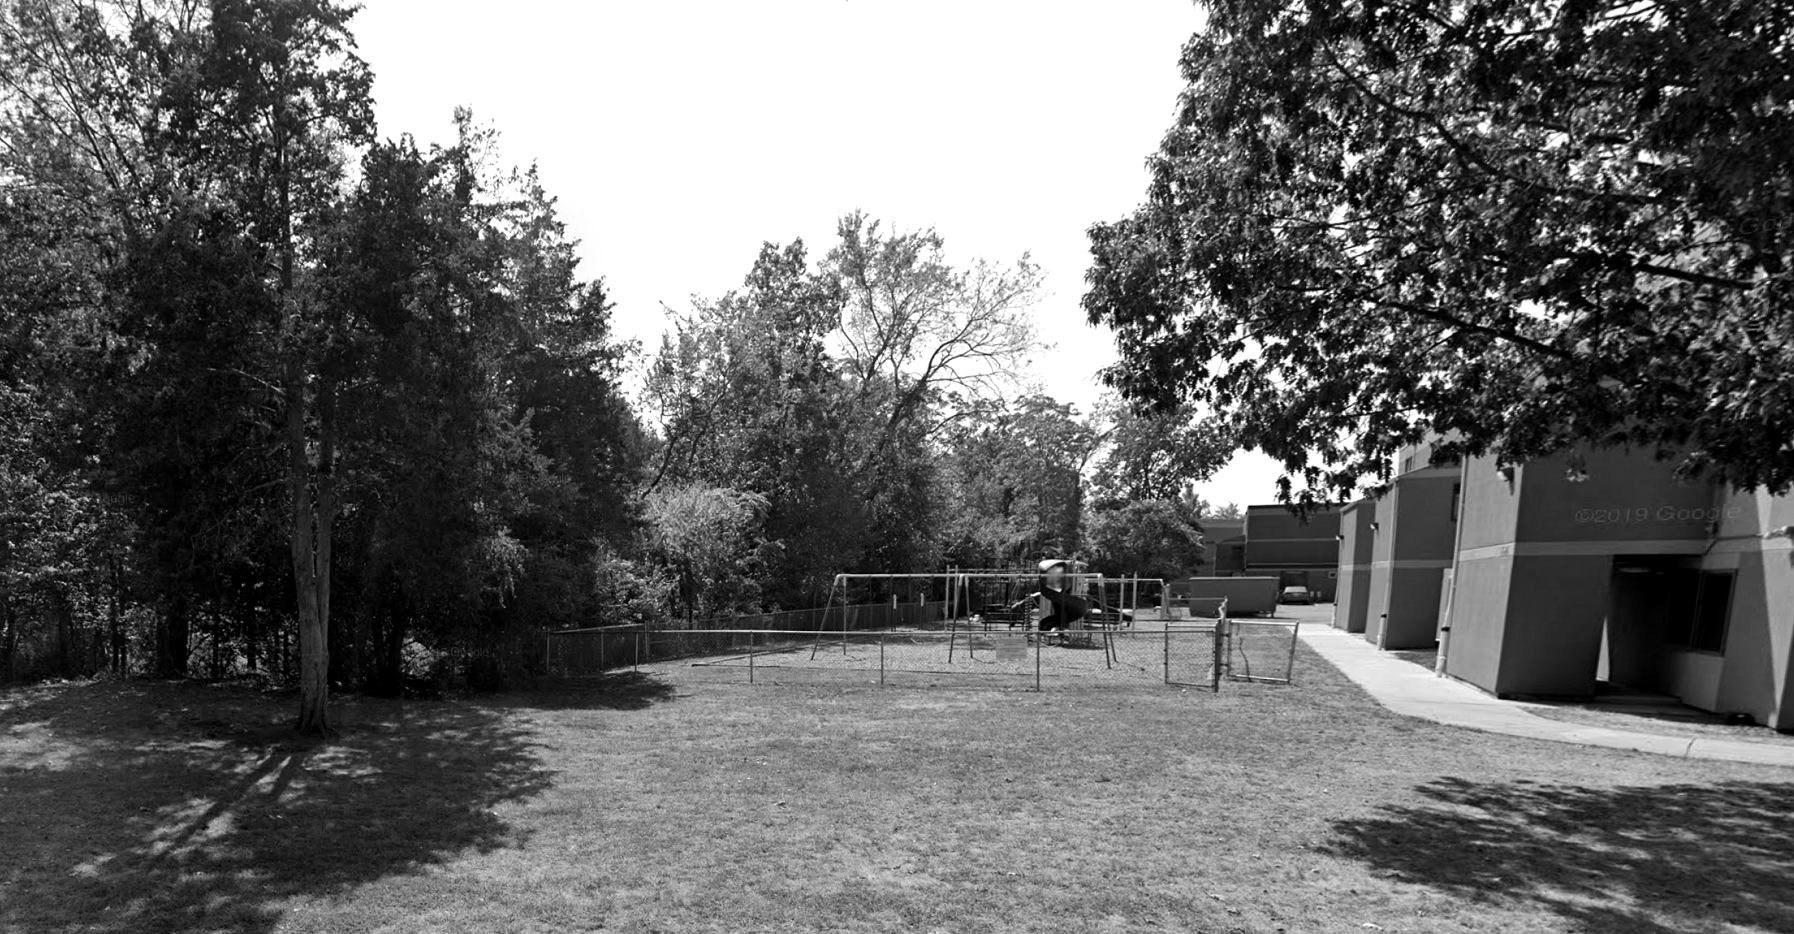
\includegraphics[height=150mm]{figures/cover_gray.png}};
  \end{scope}

  % ---- 中间：深红色的横带（页面顶端往下 164--182 mm），写英文副标题 ----
  \shade[left color=coverred!85!black, right color=coverred, opacity=0.94]
    ($(current page.north west) + (0,-164mm)$) rectangle ($(TR) + (0,-182mm)$);
  \node[anchor=east, text=white, font=\coverfont\fontsize{27}{32}\selectfont]
    at ($(TR) + (-24mm,-173mm)$) {\CoverEnSubtitle};

  % ---- 中文书名左边的空白处：一张小小的、彩色的猫狗大战，像一张贴上去的相片 ----
  % 原图 1204×772 像素，trim 裁掉底部 112 像素（水印和 START 按钮）
  \node[rotate=-5, fill=white, inner sep=1.8mm,
        drop shadow={opacity=0.4, shadow xshift=0.8mm, shadow yshift=-0.8mm}]
    at ($(current page.north west) + (52mm,-139mm)$)
    {
\includegraphics[trim=0 112 0 0, clip, width=56mm]{figures/catdog.png}};

  % ---- 右上角：竖着的红色小标签 ----
  \fill[coverred] ($(TR) + (-27mm,-18mm)$) rectangle ++(12mm,-36mm);
  \node[rotate=90, text=white, font=\coverfont\itshape\fontsize{11}{13}\selectfont]
    at ($(TR) + (-21mm,-36mm)$) {\CoverEdition};

  % ---- 上半部：作者名，下面是英文书名和中文书名，都靠右 ----
  \node[anchor=east, text=covergray, font=\coverfont\fontsize{16}{19}\selectfont]
    at ($(TR) + (-24mm,-86mm)$) {\CoverAuthor};
  \node[anchor=north east, text=black!78,
        font=\coverfont\fontsize{62}{62}\selectfont\addfontfeature{LetterSpace=3}]
    at ($(TR) + (-21mm,-94mm)$) {\CoverEnTitle};
  \node[anchor=north east, text=black!78, font=\CJKfamily{coverkai}\fontsize{44}{48}\selectfont]
    at ($(TR) + (-24mm,-124mm)$) {\CoverZhTitle};

  % ---- 左下角：“出版社”的标志 ----
  \fill[white, opacity=0.88] ($(current page.south west) + (14mm,14mm)$) rectangle ++(31mm,19mm);
  \node[text=coverred, font=\coverfont\bfseries\fontsize{30}{30}\selectfont]
    at ($(current page.south west) + (24mm,26mm)$) {C};
  \node[text=covergray, font=\coverfont\fontsize{19}{19}\selectfont]
    at ($(current page.south west) + (35.5mm,26.5mm)$) {\{\,\}};
  \node[text=covergray, font=\coverfont\fontsize{6.5}{8}\selectfont\addfontfeature{LetterSpace=10}]
    at ($(current page.south west) + (29.5mm,17.8mm)$) {LAZY PRESS};
\end{tikzpicture}
